\section{Datenorientierte Programmierung}
Das folgende Kapitel zur Datenorientierten Programmierung basiert auf dem Artikel \glqq Data-oriented design\grqq{} von Noel Llopis \cite{Data-OrientedDesign}, dem Buch \glqq Data-Oriented design\grqq{} von Richard Fabian \cite{DOD} und der Präsentation \glqq Entity Component Systems \& Data Oriented Design\grqq{} von Unity \cite{ECS-DOD}.
\subsection{Problemstellung}
\begin{figure}[H]
\begin{center}
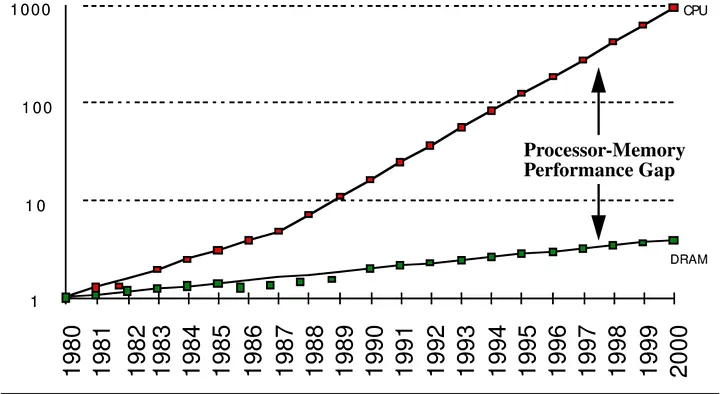
\includegraphics[scale=0.5]{Bilder/gap.png}
\caption[Performance Unterschied CPU - Speicher]{Performance Unterschied von CPU zu Speicher von 1980 bis 2000.\\
\footnotesize{Quelle: \url{http://gec.di.uminho.pt/discip/minf/ac0102/1000Gap_Proc-Mem_Speed.pdf}}}
\label{fig:gap}
\end{center}
\end{figure}
\hyperref[fig:gap]{Abbildung \ref{fig:gap}} zeigt, dass der Performance Unterschied von CPU und Speicher über die Jahre immer größer geworden ist. Dieser Trend setzt sich fort. Die zeitlichen Kosten auf dem Hauptspeicher Daten zu lesen sind wesentlich größer, als etwas auf der CPU zu berechnen. Daher wurden auch CPU's über die Zeit mit kleinen Speichereinheiten ausgerüstet um den Performanceunterschied auszugleichen - die Caches. Diese bringen den Vorteil, oft genutzte Daten direkt an der CPU zu speichern. Wenn die angefragten Daten schon im Cache liegen (Cache-Hit), benötigt der Zugriff eine wesentlich kürzere Zeit. Dennoch kommt es vor, dass die Daten nicht in dem Cache liegen (Cache-Miss). Dann braucht ein Speicherzugriff viel mehr Zeit. In der Objektorientierten Programmierung, wo meist ein Objekt nach dem anderen in den Cache geladen und verarbeitet wird, kommt dies oft vor.\\
Damit die Performance der Anwendung nicht durch Speicherzugriffe behindert wird und die gesamte Rechenleistung des Prozessors genutzt werden kann, wurde eine effizientere Lösung, das datenorientierte Design, entwickelt.
\newpage
\subsection{Datenorientiertes Design}
Im datenorientierten Design geht es vor allem um die gegebenen Daten. Wichtig hierbei sind die Fragen nach den ideale Daten für ein Problem, wie diese Daten im Speicher liegen und wer diese Daten liest oder schreibt. Der Fokus wird bei dem datenorientierten Design auf die Daten gelegt, da der Sinn von Programmen einzig und allein das Transformieren von Daten ist.\\
Die Wichtigkeit einer guten Datenstruktur wird an einem Beispiel deutlich gemacht. \hyperref[lstPersonObjektorientiert]{Listing \ref*{lstPersonObjektorientiert}} zeigt, wie im objektorientierten Design eine Person aufgebaut wäre.
\begin{lstlisting}[style=code, caption={[Person im objektorientierten Design]Person im objektorientierten Design. Objekte sind im objektorientierten Design oft Baumstrukturen, erkennbar an dem Unterobjekt \texttt{wohnort}.}, label=lstPersonObjektorientiert]
class Person {
    string name;
    Wohnort wohnort;
    int alter;
}
\end{lstlisting}
Angenommen man möchte in einem Programm aus gegebenen Personendaten das Durchschnittsalter berechnen, dann wären die gegebenen Personendaten im objektorientierten Ansatz meistens in einem Array gespeichert.
\begin{lstlisting}[style=code]
Person[] personen;
\end{lstlisting}
Um damit das Durchschnittsalter zu berechnen wäre im objektorientierten Ansatz der Zugriff auf jedes einzelne Personenobjekt nötig, um sich aus dem Objekt das Alter zu holen. Der Weg über jedes einzelne Objekt ist aber mühselig, erst recht wenn man eine größere Baumstruktur hat. Möchte man beispielsweise die Straße und Hausnummer jeder Person wissen geht der Zugriff der Daten erst über die Person und dann auf den Wohnort. Dies ist bei einer oder wenigen Personen kein Problem. Da man aber in seltenen Fällen nur wenige Objekte hat, erst recht nicht in Videospielen, ist ein anderer Ansatz hier sinnvoller. \hyperref[lstPersonenDatenorientiert]{Listing \ref*{lstPersonenDatenorientiert}} zeigt, wie im datenorientierten Design die Personen gespeichert wären.
\begin{lstlisting}[style=code, caption={[Personen im datenorientierten Design]Personen im datenorientierten Design. Die Objekte werden in ihre einzelnen Komponenten zerlegt, welche dann in Arrays gespeichert werden.}, label=lstPersonenDatenorientiert]
class Personen {
    string[] namen;
    Wohnort[] wohnorte;
    int[] alter;
}
\end{lstlisting}
Wie man sieht, wurden die Personenobjekte in ihre Komponenten zerlegt. Im datenorientierten Ansatz gibt es Objekte nur implizit. Alle Daten der Personen sind in Arrays gespeichert. Die erste Person, welche im objektorientierten Ansatz \texttt{personen[0]} ist, setzt sich im datenorientierten Ansatz aus \texttt{namen[0]}, \texttt{wohnorte[0]} und \texttt{alter[0]} zusammen. Das Durchschnittsalter lässt sich hier wesentlich einfacher berechnen. Das Array für das Alter wird in den Cache geladen, sequenziell aufaddiert und durch die Anzahl der Personen geteilt. Bei Daten, welche immer zusammen gebraucht werden ist es sinnvoll diese zusammen zu speichern, damit diese gemeinsam in den Cache geladen werden. Damit kann man sich leichter die Straße und die Hausnummer aller Personen holen, um diese weiter zu verarbeiten, falls gewünscht.\\
Das nächste Beispiel zeigt den Cachingvorteil und die damit einhergehende Performanceverbesserung.\\
\textbf{Cache Beispiel}: Angenommen es gibt Daten von zehn Personen. Der Cache ist in diesem Beispiel 64 Bytes groß. Ein Personenobjekt braucht 32 Bytes an Speicher und ein Integer (das Alter) 4 Bytes. Würde man objektorientiert vorgehen, müsste man $10 \cdot 32 = 320$ Bytes an Daten in den Cache laden und hätte dabei zehn Cache-Misses. Betrachtet man aber den datenorientierten Ansatz, müsste man nur das Alter der Personen in den Cache laden, was $10 \cdot 4 = 40$ Bytes braucht. Das gesamte Array passt in den Speicher und man hat dabei nur einen Cache-Miss.\\
\textbf{Parallelisierung}: Nicht nur die Nutzung des Caches ist ein klarer Vorteil der Datenorientierten Programmierung. Durch das Speichern einzelner Komponenten in Arrays, lässt sich die Transformierung der Daten einfacher parallelisieren. In der Objektorientierten Programmierung ist es durch Abhängigkeiten sehr umständlich Code zu parallelisieren. Im datenorientierten Ansatz kann man das Array einfach auf mehrere \textit{Threads} aufteilen und die Verarbeitung parallel ausführen.\\
\textbf{Cache Affinität}: Zusätzlich zur Parallelisierung wird der Cache bei sequenzieller Verarbeitung sehr effizient genutzt, da derselbe Code immer wieder ausgeführt wird. Wenn die Daten sequenziell verarbeitet werden resultiert das in sehr guter Performance und fast perfekter Cache Nutzung.\\
\textbf{Modularität}: Wenn objektorientierter Code zur Verbesserung der Performance angepasst wird, resultiert das oft in einem schlechter lesbarem und schlechter wartbarem Code. Das liegt an Abhängigkeiten die ein objektorientierter Ansatz oft mit sich bringt. Bei Konzentration auf die Transformierung der Daten hat man am Ende kleinere Funktionen mit weniger Abhängigkeiten zu anderem Code. Dadurch lässt sich der Code besser warten und verbessern.\\
\textbf{Testen}: Unit Tests für Objektinteraktionen können kompliziert sein. In einem objektorientierten Ansatz braucht man oft \textit{setup} und \textit{mocking} um gut testen zu können. Im datenorientierten Design sind Unit Tests jedoch einfacher. Man erstellt Eingabedaten, ruft damit die Funktion zum Testen auf und verifiziert die Ausgabedaten.\\
\textbf{Schwierigkeiten}: Das datenorientierte Design ist nicht die Lösung für alles. Es ist schwierig zu erlernen, wenn man die objektorientierte Denkweise gewohnt ist. Zusätzlich lässt es sich schwer mit bestehendem prozeduralen oder objektorientierten Code verbinden.